\chapter{Einleitung}

%% ---------------------------------------------
%% Motivation
%% ---------------------------------------------
\section{Motivation}
Lorem ipsum dolor sit amet, consetetur sadipscing elitr, sed diam nonumy eirmod tempor invidunt ut labore et dolore magna aliquyam erat, sed diam voluptua. At vero eos et accusam et justo duo dolores et ea rebum. Stet clita kasd gubergren, no sea takimata sanctus est Lorem ipsum dolor sit amet. Lorem ipsum dolor sit amet, consetetur sadipscing elitr, sed diam nonumy eirmod tempor invidunt ut labore et dolore magna aliquyam erat, sed diam voluptua. At vero eos et accusam et justo duo dolores et ea rebum. Stet clita kasd gubergren, no sea takimata sanctus est Lorem ipsum dolor sit amet.

%% ---------------------------------------------
%% Stand der Technik
%% ---------------------------------------------
\section{Stand der Technik}
Lorem ipsum dolor sit amet, consetetur sadipscing elitr, sed diam nonumy eirmod tempor invidunt ut labore et dolore magna aliquyam erat, sed diam voluptua. At vero eos et accusam et justo duo dolores et ea rebum. Stet clita kasd gubergren, no sea takimata sanctus est Lorem ipsum dolor sit amet. Lorem ipsum dolor sit amet, consetetur sadipscing elitr, sed diam nonumy eirmod tempor invidunt ut labore et dolore magna aliquyam erat, sed diam voluptua. At vero eos et accusam et justo duo dolores et ea rebum. Stet clita kasd gubergren, no sea takimata sanctus est Lorem ipsum dolor sit amet.

... Siehe Abbildung \ref{fig_example}.

\begin{figure}[h!]
    \centering
    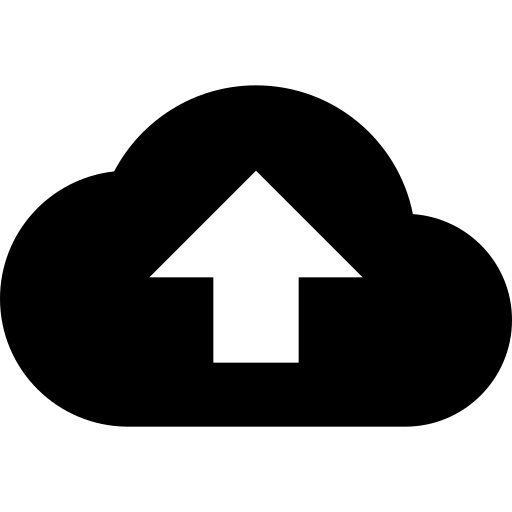
\includegraphics[width=\textwidth]{img/example_image.png}
    \caption{Ein wundervolles Bild in ganzer Breite}
    \label{fig_example}
\end{figure}

... Siehe Abbildung \ref{fig_example_halfsize}

\begin{figure}[h!]
    \centering
    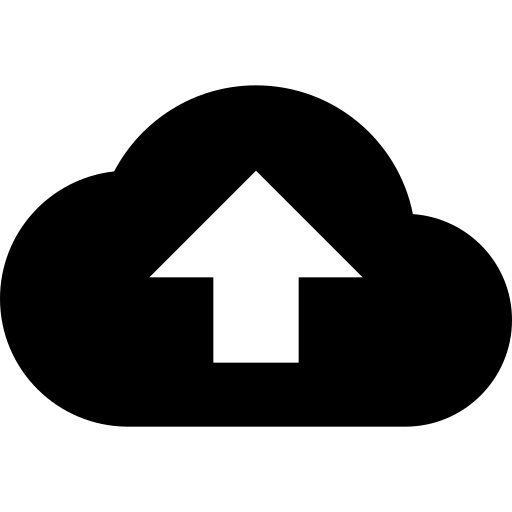
\includegraphics[width=0.5\textwidth]{img/example_image.png}
    \caption[Kurzbeschreibung für Abbildungsverzeichnis]{Ein wundervolles Bild in 50\% Breite}
    \label{fig_example_halfsize}
\end{figure}

... in Tabelle \ref{tbl_example_table} ...

\begin{table}[!h]
    \centering
    \begin{tabular}{l|ll}
        Datensatz 1     & Wert 1    & Einheit \\
        Datensatz 2     & Wert 2    & Einheit \\ \hline
        $\sum$          & Summe     & Einheit \\
    \end{tabular}
    \caption{Beispiel für eine Tabelle}
    \label{tbl_example_table}
\end{table}

Quellcode:

\begin{minted}{json}
{   
    "id" : 1234,  
    "field1": "hallo",  
    "field2" : "welt"
}
\end{minted}

Quellcode kann aber auch beipsielsweise in einer Zeile mit Text stehen: \mintinline{python}{print(x**2)} und so weiter.


%% ---------------------------------------------
%% Zielsetzung
%% ---------------------------------------------
\section{Zielsetzung}
Lorem ipsum dolor sit amet, consetetur sadipscing elitr, sed diam nonumy eirmod tempor invidunt ut labore et dolore magna aliquyam erat, sed diam voluptua. At vero eos et accusam et justo duo dolores et ea rebum. Stet clita kasd gubergren, no sea takimata sanctus est Lorem ipsum dolor sit amet. Lorem ipsum dolor sit amet, consetetur sadipscing elitr, sed diam nonumy eirmod tempor invidunt ut labore et dolore magna aliquyam erat, sed diam voluptua. At vero eos et accusam et justo duo dolores et ea rebum. Stet clita kasd gubergren, no sea takimata sanctus est Lorem ipsum dolor sit amet. \cite{Nobody07}

%% ---------------------------------------------
%% Aufbau der Projektarbeit
%% ---------------------------------------------
\section{Aufbau der \myworktype}
Lorem ipsum dolor sit amet, consetetur sadipscing elitr, sed diam nonumy eirmod tempor invidunt ut labore et dolore magna aliquyam erat, sed diam voluptua. At vero eos et accusam et justo duo dolores et ea rebum. Stet clita kasd gubergren, no sea takimata sanctus est Lorem ipsum dolor sit amet. Lorem ipsum dolor sit amet, consetetur sadipscing elitr, sed diam nonumy eirmod tempor invidunt ut labore et dolore magna aliquyam erat, sed diam voluptua. At vero eos et accusam et justo duo dolores et ea rebum. Stet clita kasd gubergren, no sea takimata sanctus est Lorem ipsum dolor sit amet. \cite{Nobody06}
